\documentclass[a4paper]{article}
\usepackage[pdftex]{hyperref}
\usepackage[latin1]{inputenc}
\usepackage[english]{babel}
\usepackage{a4wide}
\usepackage{amsmath}
\usepackage{amssymb}
\usepackage{algorithmic}
\usepackage{algorithm}
\usepackage{ifthen}
\usepackage{listings}
% move the asterisk at the right position
\lstset{basicstyle=\ttfamily,tabsize=4,literate={*}{${}^*{}$}1}
%\lstset{language=C,basicstyle=\ttfamily}
\usepackage{moreverb}
\usepackage{palatino}
\usepackage{multicol}
\usepackage{tabularx}
\usepackage{comment}
\usepackage{verbatim}
\usepackage{color}

% Because of an error on line 41 I added this
\usepackage{graphicx}

% Used for drawing DFAs and NFAs
\usepackage{tikz}
\usetikzlibrary{automata, positioning}

% Defined checkmark sign
\def\checkmark{\tikz\fill[scale=0.4](0,.35) -- (.25,0) -- (1,.7) -- (.25,.15) -- cycle;}

% Table coloring
\usepackage{color, colortbl}
\usepackage[first=0,last=9]{lcg}

% Tab
\newcommand\tab[1][1.15cm]{\hspace*{#1}}

%% pdflatex?
\newif\ifpdf
\ifx\pdfoutput\undefined
\pdffalse % we are not running PDFLaTeX
\else
\pdfoutput=1 % we are running PDFLaTeX
\pdftrue
\fi
%\ifpdf
%\usepackage[pdftex]{graphicx}
%\else
%\usepackage{graphicx}
%\fi
\ifpdf
\DeclareGraphicsExtensions{.pdf, .jpg}
\else
\DeclareGraphicsExtensions{.eps, .jpg}
\fi

\parindent=0cm
\parskip=0cm

\setlength{\columnseprule}{0.4pt}
\addtolength{\columnsep}{2pt}

\addtolength{\textheight}{5.5cm}
\addtolength{\topmargin}{-26mm}
\pagestyle{empty}

%%
%% Sheet setup
%% 
\newcommand{\coursename}{Computability and Complexity}
\newcommand{\courseno}{CO21-320352}
 
\newcommand{\sheettitle}{Homework}
\newcommand{\mytitle}{}
\newcommand{\mytoday}{February 26th, 2019}

% Current Assignment number
\newcounter{assignmentno}
\setcounter{assignmentno}{3}

% Current Problem number, should always start at 1
\newcounter{problemno}
\setcounter{problemno}{1}

%%
%% problem and bonus environment
%%
\newcounter{probcalc}
\newcommand{\exercise}[2]{
  \pagebreak[2]
  \setcounter{probcalc}{#2}
  ~\\
  {\large \textbf{Exercise \arabic{problemno}} \hspace{0.2cm}\textit{#1}} \refstepcounter{problemno}\vspace{2pt}\\}

\newcommand{\bonus}[2]{
  \pagebreak[2]
  \setcounter{probcalc}{#2}
  ~\\
  {\large \textbf{Bonus Problem \textcolor{blue}{\arabic{assignmentno}}.\textcolor{blue}{\arabic{problemno}}} \hspace{0.2cm}\textit{#1}} \refstepcounter{problemno}\vspace{2pt}\\}

%% some counters  
\newcommand{\assignment}{\arabic{assignmentno}}

%% solution  
\newcommand{\solution}{\pagebreak[2]{\bf Solution:}\\}

%% Hyperref Setup
\hypersetup{pdftitle={Homework \assignment},
  pdfsubject={\coursename},
  pdfauthor={},
  pdfcreator={},
  pdfkeywords={Computability and Complexity},
  %  pdfpagemode={FullScreen},
  %colorlinks=true,
  %bookmarks=true,
  %hyperindex=true,
  bookmarksopen=false,
  bookmarksnumbered=true,
  breaklinks=true,
  %urlcolor=darkblue
  urlbordercolor={0 0 0.7}
}

\begin{document}
\coursename \hfill Course: \courseno\\
Jacobs University Bremen \hfill \mytoday\\
Dragi Kamov and Dushan Terzikj\hfill
\vspace*{0.3cm}\\
\begin{center}
{\Large \sheettitle{} \assignment\\}
\end{center}

\exercise{}{0}
\solution
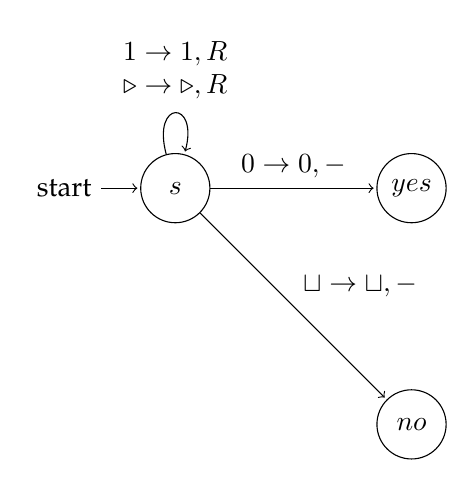
\begin{tikzpicture}[shorten >=1pt,node distance=3cm,on grid,auto]
   \node[state,initial] (0) {$ s $};
   \node[state] (1) [right=of 0] {$ yes $};
   \node[state] (2) [below=of 1] {$ no $};
   \path[->]
    (0) edge                    node {$ 0 \rightarrow 0, -$} (1)
    (0) edge                    node {$ \sqcup \rightarrow \sqcup, - $} (2)
    (0) edge [loop above]       node {$ \begin{matrix}1 \rightarrow 1, R \\ \triangleright \rightarrow \triangleright, R \end{matrix} $} (0);
\end{tikzpicture}
\begin{center}
    \begin{tabular}{|c|c|c|} \hline
        p $ \in $ K & $ \sigma \in \Sigma $ & $ \delta $(p, $ \sigma $)  \\ \hline
        s & 0 & (yes, 0, -) \\ \hline
        s & 1 & (s, 1, $ \rightarrow $) \\ \hline
        s & $ \sqcup $ & (no , $ \sqcup $, -) \\ \hline
        s & $ \triangleright $ & (s, $ \triangleright $, $ \rightarrow $) \\ \hline
    \end{tabular}
\end{center}
This language goes through the tape and checks if there is a 0 on the tape, if there is then it goes to the accepting state \textit{yes}, and if there is no 0 on the tape the it reaches the $ \sqcup $ and it goes to the rejecting state \textit{no}. \\ \\
The RAM program would look like this:
\begin{enumerate}
    \item[\textcolor{gray}{1}] read
    \item[\textcolor{gray}{2}] if c(0) = 0 goto 5
    \item[\textcolor{gray}{3}] if c(0) = $ \sqcup $ goto 6
    \item[\textcolor{gray}{4}] goto 1
    \item[\textcolor{gray}{5}] store 1 goto 7
    \item[\textcolor{gray}{6}] store 0
    \item[\textcolor{gray}{7}] end
\end{enumerate}

\exercise{}{0}
\solution
For the sake of beautiful mathematical notation, let us define the function $plus2$ as $\pi_2$.\\ \\
We already know that the successor function $\sigma$ is a primitive recursive function. Let's use rule (4) from the lecture notes, make a setting and combine it with the successor function.\\ \\
Let $r=m=1$, then we have the functions $f:N^r\rightarrow N$, $g:N^m\rightarrow N$ and $h:N^r\rightarrow N$. If we set $f=g=\sigma$ and $h=\pi_2$ and using rule (4) from the lecture notes (substituting) we have:
\begin{align*}
    &h(n)=f(g_1(n),..., g_r(n))\\
    \Rightarrow &\pi_2(n)=\sigma (\sigma (n))\\
    \Rightarrow &\pi_2(n)=n+2
\end{align*}

\newpage
\exercise{}{0}
\solution
Let's define our function more "mathematically":\\ \\
\[ 
\pi_{-1}(n)= \left\{
\begin{array}{ll}
      0 & n=0\\
      n-1 & \text{otherwise}
\end{array} 
\right. 
\]\\ \\
We already know that the projection function $p_i^k$ ("rule" 3 from lecture notes) and the null function \textbf{O} ("rule" 1 from lecture notes) are primitive recursive functions. We can use those 2 functions along with the (5) "rule" from the lecture notes to form a proof that $pi_{-1}$ is also primitive recursive. Observe:\\ \\
If we set $r=0$, then we have the functions $f:N^r\rightarrow N$, $g:N^{r+2}\rightarrow N$ and $h:N^{r+1}\rightarrow N$. According to "rule" (5) from the lecture notes, we have:
\begin{align}
    h(0)&=f()\\
    h(n+1)&=g(n, h(n))
\end{align}
Before we go any further, we can write (2) from above as $h(n)=g(n-1, h(n-1))$.  
Now we can make the setting:
\begin{center}
    $h=\pi_{-1}$\\$g(n, m)=p_1^2(n, m)$\\$f()=\text{\textbf{O}}()$
\end{center}
Once we substitute, we have:
\[ 
\pi_{-1}(n)= \left\{
\begin{array}{ll}
      \text{\textbf{O}}() & n=0\\
      p_1^2(n-1, \pi_{-1}(n-1)) & \text{otherwise}
\end{array} 
\right. 
\]

\end{document}